\item \textbf{Iron Ears: Data Structure}

\textit{Iron Ears} é um jogo do gênero \textit{puzzle}, desenvolvido pela
\textit{NPC42 Games}, com o objetivo de ensinar conceitos de estruturas de
dados de forma interativa. Ambientado em um universo fictício habitado por
animais antropomorfizados, com inteligência e racionalidade comparáveis às
humanas.

O jogo coloca o jogador no papel de um coelho humanóide encarregado de
projetar e operar linhas de montagem de \textit{Mechs}. Esses robôs são
essenciais na resistência contra uma facção hostil que busca dominar o mundo.

A mecânica do jogo integra diretamente estruturas de dados clássicas, como
listas, filas e pilhas, aos sistemas de produção, exigindo que o jogador
aplique esses conceitos para resolver desafios e otimizar os processos de
fabricação. \cite{IronEarsItchio}

\begin{figure}[H]
	\centering
	\caption{Captura de tela do jogo Iron Ears}
	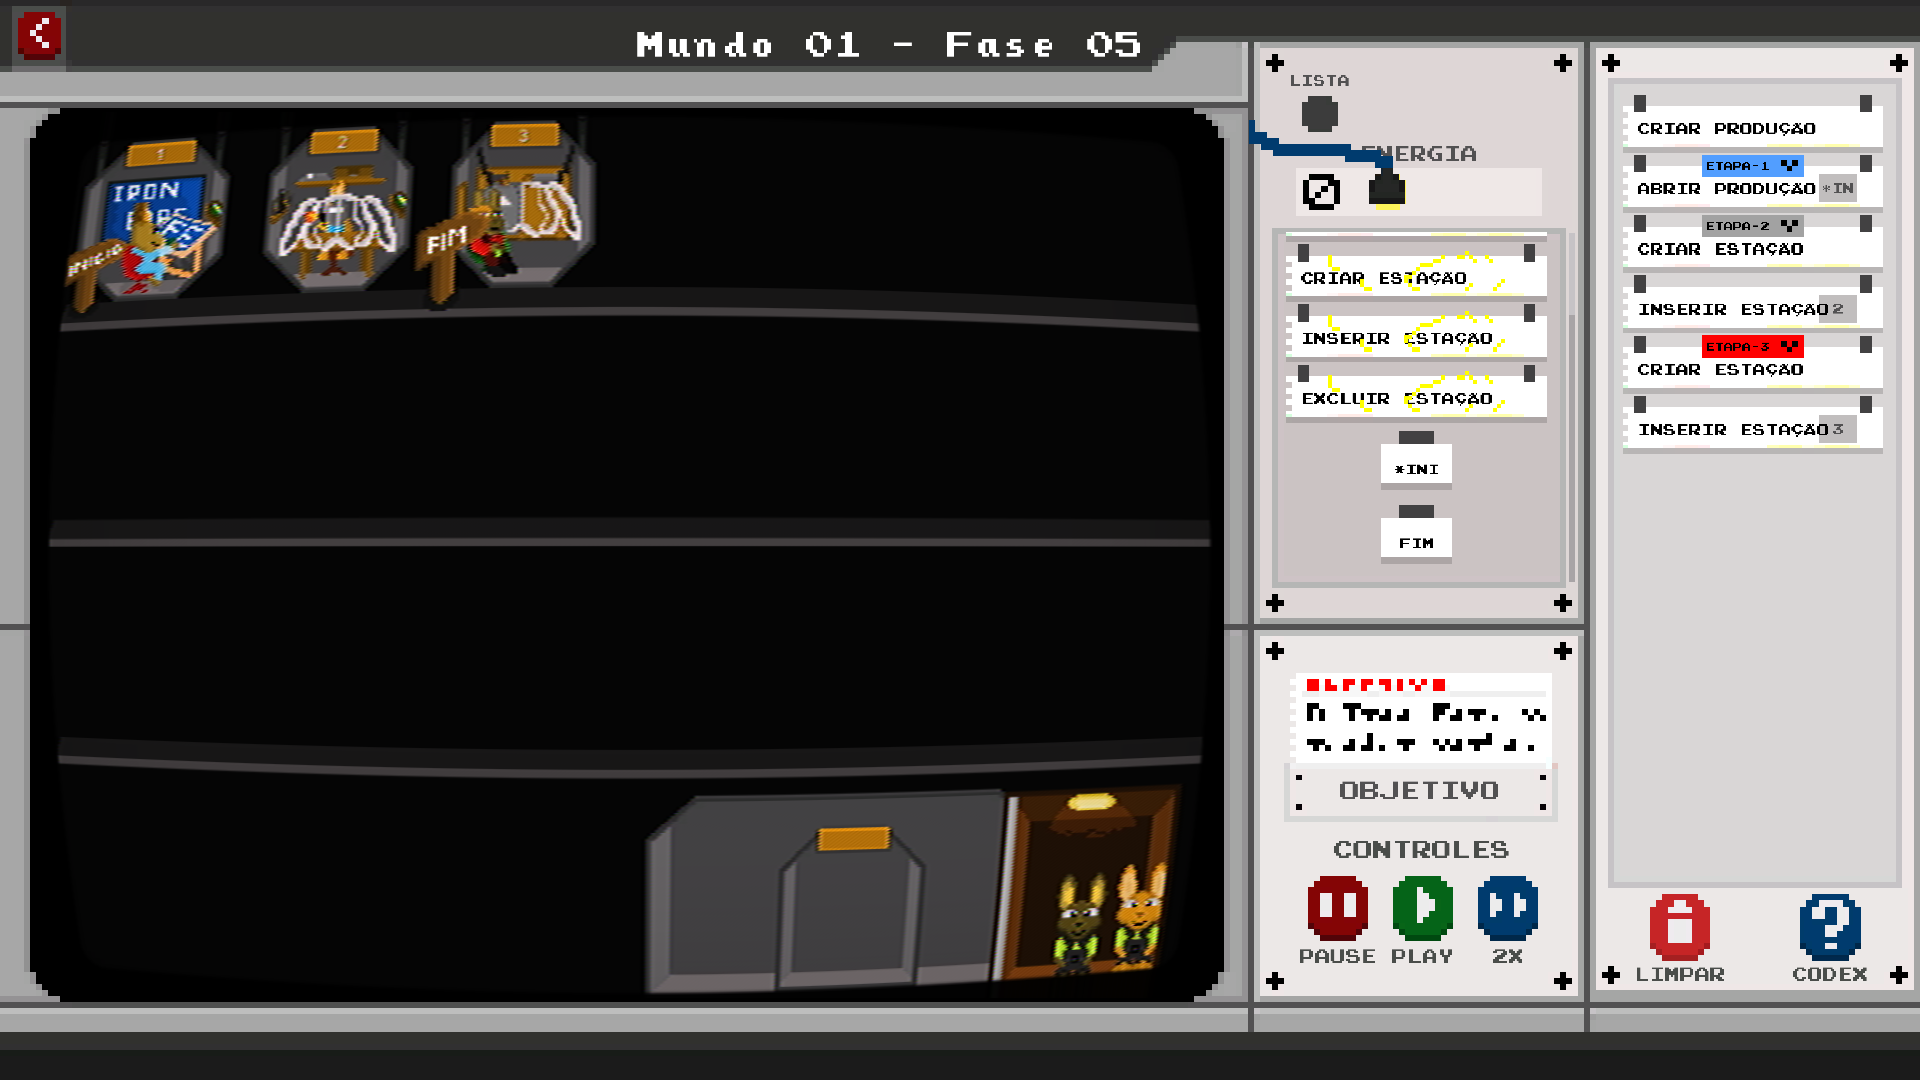
\includegraphics[width=0.8\textwidth]{images/iron-ears.png}
	\legend{Fonte: \cite{IronEarsItchio}}
	\label{fig:ie}
\end{figure}

